\documentclass[10pt]{article}
\usepackage{sdss2020}
\usepackage{url}
\usepackage{latexsym}
\usepackage{amsmath, amsthm, amsfonts}
\usepackage{algorithm, algorithmic}  
\usepackage{graphicx}
\usepackage{booktabs}
\usepackage{multirow}
\usepackage{float}
\usepackage[spanish]{babel}
\usepackage{hyperref}
\usepackage[utf8]{inputenc}

\title{
    PÉNDULOS ACOPLADOS\\
    Universidad del Valle \\
    Departamento de Física, experimentación en Física III
}

\author{
    Nicolás Aguilera García \\
    {\tt 2021273030} \\
    \And
    Andrés Felipe Valencia Fonseca \\
    {\tt 202125166} \\
    \And
    Kevin Giraldo Hincapie\\
    {\tt 202024236} \\
}

\date{}




\begin{document}
    \maketitle

    \begin{abstract}
        En esta práctica de laboratorio se analiza el comportamiento de un sistema de dos péndulos acoplados mediante el resorte, esto con el fin de determinar experimentalmente las frecuencias de los modos normales del sistema junto con los valores para constantes como la gravedad y la constante de elasticidad del resorte. Tras el análisis realizado se logró determinar que $g = 11.68 \pm 1.82$ y $k = 2.811 \pm 0.78$.

            {\bf Keywords: } Péndulo acoplado, resorte, oscilaciones, frecuencia.
    \end{abstract}

    \section{Análisis de datos}
        Partiendo de los datos recolectados mediante el instrumento de \texttt{CASSY Labs} se desarrolló un trabajo estadístico en el lenguaje \texttt{python} y con ayuda de diferentes librerías como \texttt{numpy} y \texttt{scipy} para realizar las regresiones. El conjunto total de datos se puede ver en \href{https://drive.google.com/drive/folders/1HW9HpYB_uKflT2-5fgyOxWJDfALd5ZZW?usp=share_link}{\texttt{drive}}, a continuación solo se presentarán los resultados más relevantes.

        El total de mediciones llevadas a cabo fue de 12, 6 para oscilaciones llevadas a cabo en el modo normal de fase y las restantes realizadas en contrafase, de donde, la gráfica que presenta el movimiento oscilatorio del sistema, para todos los casos está dado por lo que se puede observar en las siguientes gráficas.

        \begin{figure}[H]
            \centering
            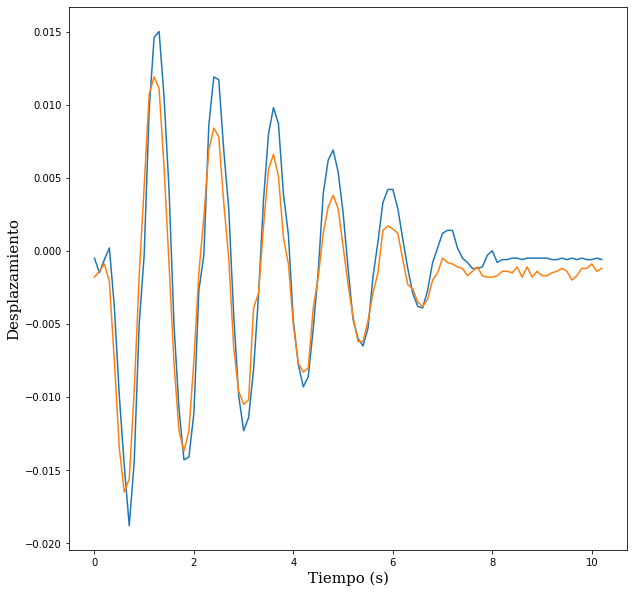
\includegraphics[scale = 0.3]{img/diagrama_fase.png}
            \caption{Evolución del desplazamiento del péndulo en fase.}
        \end{figure}

        \begin{figure}[H]
            \centering
            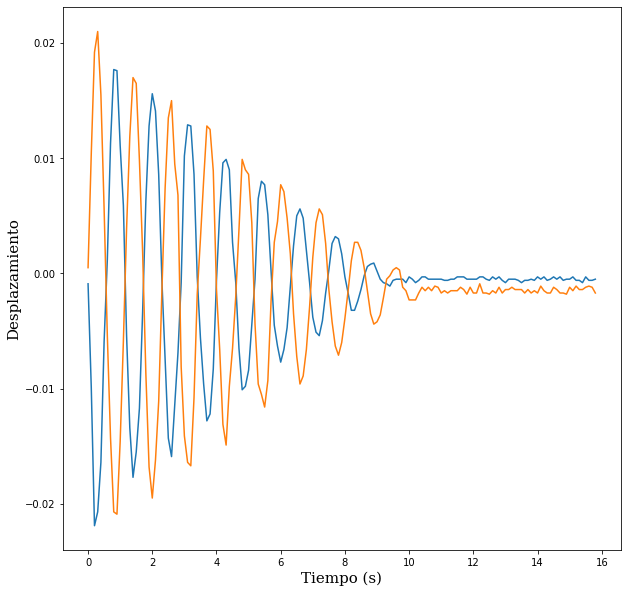
\includegraphics[scale = 0.3]{img/digrama_desfase.png}
            \caption{Evolución del desplazamiento del péndulo en desfase.}
        \end{figure}
 
        Para cada uno de los casos anteriores se determinó el valor de la frecuencia natural del sistema, realizado mediante la búsqueda de los máximos con ayuda de \texttt{python} para determinar el periodo y a continuación determinar las frecuencias de la forma $ w = 2 \pi / T $. Estos resultados se pueden observar en la tabla \ref{datatable} donde se encuentra además la relación ($ \epsilon $) entre la longitud del péndulo y la altura a la que se encontraba el resorte durante dicha medición.
 
        \begin{table}[H]
            \centering
            \begin{tabular}{|c|ll|ll|ll|}
            \hline
            \multirow{2}{*}{\textbf{$l$}} & \multicolumn{2}{c|}{\textbf{$w_1$}}                                      & \multicolumn{2}{c|}{\textbf{$w_2$}}                                      & \multicolumn{2}{c|}{\textbf{$ \epsilon $}}                                       \\ \cline{2-7} 
                                                        & \multicolumn{1}{c|}{\textbf{$val$}} & \multicolumn{1}{c|}{\textbf{$\pm\delta$}} & \multicolumn{1}{c|}{\textbf{$val$}} & \multicolumn{1}{c|}{\textbf{$\pm\delta$}} & \multicolumn{1}{c|}{\textbf{$val$}} & \multicolumn{1}{c|}{\textbf{$\pm\delta$}} \\ \hline
            6.0                                         & \multicolumn{1}{l|}{5.35}         & 0.42                              & \multicolumn{1}{l|}{5.40}         & 0.42                              & \multicolumn{1}{l|}{0.15}         & 0.001                             \\ \hline
            11.5                                        & \multicolumn{1}{l|}{5.35}         & 0.42                              & \multicolumn{1}{l|}{5.87}         & 0.50                              & \multicolumn{1}{l|}{0.29}         & 0.001                             \\ \hline
            13.8                                        & \multicolumn{1}{l|}{5.34}         & 0.41                              & \multicolumn{1}{l|}{6.13}         & 0.54                              & \multicolumn{1}{l|}{0.35}         & 0.001                             \\ \hline
            21.5                                        & \multicolumn{1}{l|}{5.32}         & 0.41                              & \multicolumn{1}{l|}{6.87}         & 0.67                              & \multicolumn{1}{l|}{0.54}         & 0.001                             \\ \hline
            26.5                                        & \multicolumn{1}{l|}{5.31}         & 0.41                              & \multicolumn{1}{l|}{7.46}         & 0.79                              & \multicolumn{1}{l|}{0.67}         & 0.001                             \\ \hline
            29.5                                        & \multicolumn{1}{l|}{5.38}         & 0.42                              & \multicolumn{1}{l|}{7.72}         & 0.84                              & \multicolumn{1}{l|}{0.75}         & 0.001                             \\ \hline
            \end{tabular}
            \caption{Valores experimentales obtenidos para $w_1$, $w_2$ y $\epsilon$.}
            \label{datatable}
        \end{table}

        Ahora, conociendo el valor experimental de la frecuencia correspondiente al modo normal de contrafase $ w_2 $ junto con $ \epsilon $ se realiza la gráfica de $ w_2^2 vs \epsilon^2 $ la cual mediante la propia definición teórica de $ w_2 $

        \begin{equation}
            w_2^2 = \frac{g}{L} + 2 \epsilon^2 \frac{k}{M}
        \end{equation}

        se pueden determinar los valores para la gravedad y la constante de elasticidad del resorte al relacionar la pendiente y el intercepto de la regresión lineal que mejor se ajuste a los datos.

        \begin{figure}[H]
            \centering
            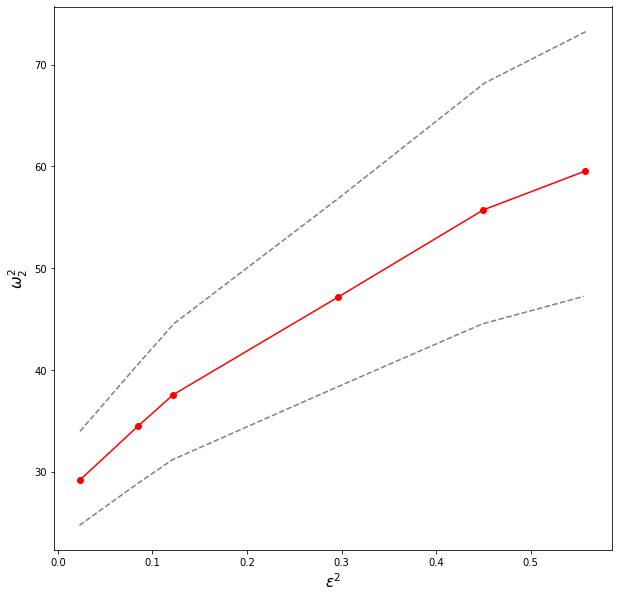
\includegraphics[scale = 0.3]{img/omaga_vs_epsilon.png}
            \caption{Grafica de $w_2^2 \: vs \: \epsilon^2$.}
        \end{figure}

        Con lo cual los valores para $g$ y $k$ se encuentran dados por:

        \begin{itemize}
            \item $g = 11.68 \pm 1.82$
            \item $k = 2.811 \pm 0.78$
        \end{itemize}

        Los valores de error al comparar los resultados experimentales con los teóricos ($g = 9.8099$ y $k=2.9754$) se encuentran dados por:

        \begin{itemize}
            \item \% de error para $g$ es de $19.06\%$
            \item \% de error para $k$ es de $5.52\%$
        \end{itemize}

    \section{Conclusiones}
        De los valores obtenidos para la gravedad y la constante de elasticidad del resorte, se puede observar que los valores, aunque no exactos, son cercanos y con un bajo error respecto al valor real, por lo menos en el caso de la constante $k$, ya que el valor de la gravedad cuenta con un mayor error aunque el valor teórico este dentro de la incertidumbre de la medición.

        Si bien el tratamiento tórico llevado a cabo es el aplicable a modelos de sistemas no amortiguados, el sistema experimental realmente trabajado si cuenta con amortiguamiento, como se pudo observar en las gráficas anteriormente presentadas, más sin embargo, por los valores experimentales obtenidos para la gravedad y la constante de elasticidad del resorte que aunque como se discutió anteriormente no son del todo certeros se puede decir que la simplificación del modelo realizado para el sistema es válida y permite obtener buenos resultados sin un extenso trabajo teórico.
\end{document}
